\section{Durchführung und Aufbau}
\label{sec:Durchführung}

\begin{figure}[H]
  \centering
  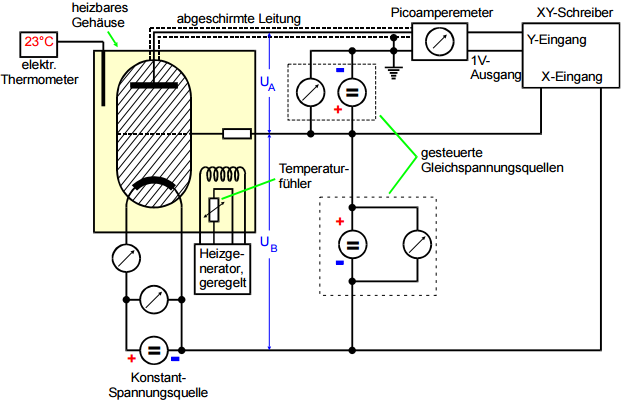
\includegraphics[height=7cm]{picture/Schaltung}
  \caption{Schaltung zur Aufnahme der Franck-Hertz-Kurve. \cite[10]{sample}}
  \label{fig:Schaltung}
\end{figure}

Nun wird der XY-Schreiber so eingestellt, dass dieser in der unteren linken Ecke des Millimeterpapiers beginnt. Dazu werden die Knöpfe "Zero" an dem Schreiber verwendet. Außerdem soll für jede Kurve ein neues Millimeterpapier eingelegt werden. Nun wird die in Abbildung \eqref{fig:Schaltung} zu sehende Schaltung aufgebaut. Die Gleichspannungsquellen können in einer vorgegebenen Zeit ihren vollen Ausschlagsbereich durchlaufen (Sweap). Dabei wird der Auffängerstrom $I_\text{A}$ von einem Picoamperemeter ausgelesen und auf den y-Eingang eines XY-Schreiber gegeben. An den x-Eingang wird entweder die Brems- oder die Beschleunigungsspannung angelegt. \\
Zu erst wird die \textbf{integrale Energieverteilung} aufgenommen. Dafür wird für verschiedene Temperaturen ($T \approx 20\,\text{°C und } T = 140\,\text{°C} - 160\,\text{°C}$) die Bremsspannung gegen den Auffängerstrom aufgetragen. Die Beschleunigungsspannung wird auf 11\,V gestellt und für jede Temperatur wird die Bremsspannung von 0\,V bis 10\,V laufen gelassen. Die Verstärkung des Schreibers wird so eingestellt, dass die Kurve so groß wie möglich zu erkennen ist ohne das etwas abgeschnitten ist. \\
Als zweites wird die \textbf{Franck-Hertz-Kurve} aufgenommen. Dazu wird nun die Beschleunigungsspannung an den Schreiber angeschlossen und die Bremsspannung auf 1\,V eingestellt. Für verschiedene Temperaturen ($T = 160\,\text{°C} - 200\,\text{°C}$) soll nun die Beschleunigugsspannung gleichmäßig von 0\,V bis 60\,V aufgedreht werden. Für die Verstärkung des Schreiber gilt wieder, eine möglichst große Kurve ohne etwas abzuschneiden. \\
Zu letzt wird die \textbf{Ionisierungsspannung} von Quecksilber untersucht. Dazu wird die Bremsspannung auf auf -30\,V gestellt und die Temperatur wird zwischen $T = 100\,\text{°C} - 110\,\text{°C}$ gehalten. Die Beschleunigungsspannung wird von 0\,V bis 60\,V laufen gelassen.
